\documentclass[11pt,letterpaper]{article}
\usepackage{floatrow}
\usepackage{amsmath}
\usepackage{amsthm}
\usepackage{amssymb}
\usepackage{amsfonts}
\usepackage{color}
%\usepackage{hyperref}
\usepackage{algorithm}
\usepackage{caption}
\usepackage{MnSymbol}
\usepackage{url}
\usepackage[margin=1in]{geometry}
\usepackage[labelfont=bf,font=small,margin=1em]{caption} %font of captions
\usepackage{mathtools}
\usepackage{refcount}
\usepackage[shortlabels]{enumitem}

\usepackage{tikz}
\usetikzlibrary{shapes,snakes}
\usetikzlibrary{arrows.meta,automata,positioning,arrows}

\newcommand{\Z}{\mathbb{Z}}
\newcommand{\N}{\mathbb{N}}
\newcommand{\C}{\mathbb{C}}
\newcommand{\R}{\mathbb{R}}
\newcommand{\Q}{\mathbb{Q}}
\renewcommand{\Pr}[1]{{\mathop{\text{Pr}}\left[#1\right]}}
\newcommand{\Ex}[1]{{\mathop{\mathbb{E}}\left[#1\right]}}
\newcommand{\todo}[1]{{\bf \color{red} TODO: #1}}

\newtheorem*{claim}{Claim}
\newtheorem{theorem}{Theorem}
\newtheorem{lemma}[theorem]{Lemma}
\newtheorem{corollary}[theorem]{Corollary}
\newtheorem{conjecture}[theorem]{Conjecture}
\newtheorem{proposition}[theorem]{Proposition}
\newtheorem{definition}[theorem]{Definition}
\newtheorem{notation}[theorem]{Notation}
\newtheorem{example}[theorem]{Example}
\newtheorem{remark}[theorem]{Remark}
\newtheorem{problem}[theorem]{Problem}
\newtheorem{acknowledgment}[]{Acknowledgment}

\title{}
\author{}
\date{\today}

\begin{document}
\maketitle

Jamal owns a new ride-hailing business. His business operates in the following way: at least $12$ hours before a trip is desired, a customer orders a trip from a starting location to an ending location to take place at a specified starting time. Although Jamal has considered ride-sharing in the past, due to the ongoing pandemic, each ordered trip is currently completed before another begins. Jamal’s company has a layout of the current service area and upper bounds for the time required to drive any particular road. At some point, the team would like to incorporate traffic data to make the map dynamic, but at the moment fixed costs are what we have to work with.

By having each trip scheduled in advance, Jamal’s company is able to optimize route-planning and provide an attractive business model for drivers. His company does this in the following way: Every $8$ hours, Jamal selects a set of drivers to work a shift picking up and dropping off customers according to their desired schedules. Drivers are then paid per shift worked, rather than per trip completed. Jamal has found this model to be more satisfactory to drivers compared to current ride-hailing businesses. In current businesses, drivers face uncertainty as to how many rides they will be able to procure, and thus how much money they will earn. Jamal’s business, on the other hand, pays drivers for every shift they work, and so a driver will either be earning money (if they work a shift) or be free to occupy their time by other means (if they aren’t needed for a shift), instead of waiting around in their car hoping for a passenger to request a ride.

Unfortunately, Jamal is more of a business-type and needs help with coding for his company. In particular, he is lacking the algorithm to determine given a set of ordered trips in an eight-hour window, the minimum number of drivers that should be hired for the given shift. Can you help Jamal with this crucial task?

\begin{figure}[h]
	\begin{center}
		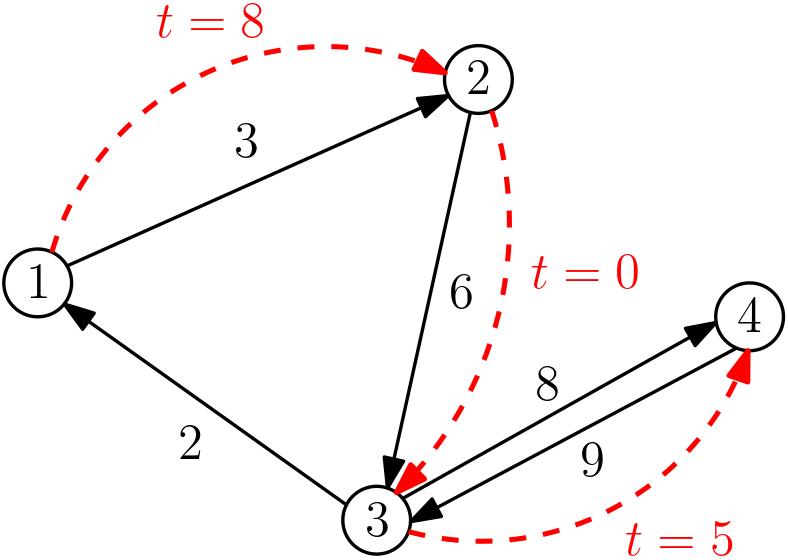
\includegraphics[scale=0.3]{sample-graph.png}
	\end{center}
	\caption{Illustration of sample input. Scheduled trips are depicted in dashed red lines with their respective start times. The optimal solution is to have one driver complete the trip from $2$ to $3$ at time $0$, then travel to location $1$ arriving at time $8$, and then complete the trip from $1$ to $2$. The second driver can complete the trip from $3$ to $4$.}
	\label{fig:sample}
\end{figure}

\section*{Input}
Input will begin with three integers on one line: $n$ ($2 \leq n \leq 100$), the number of pickup or destination locations in the model of the service area, $m$ ($1 \leq m \leq n*(n-1)$), the number of one-directional roads in the service area, and $k$ ($1 \leq k \leq 1000$), the number of requested trips that must be fulfilled. The next $m$ lines each contain three integers $u$, $v$, and $w$ ($1 \leq u,v \leq n$, $u \neq v$, $1 \leq w < 480$), indicating there is a road from location $u$ to location $v$ that takes $w$ minutes to travel. Between any two locations $u$ and $v$, there can be a road from $u$ to $v$ and from $v$ to $u$ but there will be at most one road in one direction between any two locations. The next $k$ lines each contain three integers $u$, $v$, and $t$ ($1 \leq u,v \leq n$, $u \neq v$, $0 \leq t < 480$), indicating there is a trip requested from location $u$ to location $v$ departing location $u$ at minute $t$. There can be multiple trips requested from the same starting locations at the same time or arriving at the same ending locations at the same time. It is guaranteed every location is accessible from any other location.

\section*{Output}
Output a single integer representing the minimum number of drivers that must be hired for this shift to complete all trips. Roads can be used by as many drivers as required. Assume pickup and drop-off takes $0$ minutes. Picking up or dropping off at the same location does not delay trips. Assume hired drivers can drive to any starting location so they are ready to pick up any trip at minute $0$ and are willing to complete trips requested before minute $480$ that finish on or after minute $480$. Customers must be picked up exactly at their desired pickup time.


\bibliographystyle{alpha}
\bibliography{ref}

\end{document}

